% !TeX program = pdflatex
% AntiFLipper v9 -- reframed around AntiFLipper-CC and the report-faking attacker.
% Result tables/figures are produced by make_results.py from Code_Journal_Experiments;
% run `python make_results.py` and recompile after the experiments finish.
\documentclass[conference]{IEEEtran}

\usepackage{amsmath,amssymb,amsfonts}
\usepackage{graphicx}
\usepackage{multirow}
\usepackage{xcolor}
\usepackage{url}
\usepackage[ruled,vlined,linesnumbered]{algorithm2e}
\usepackage{cite}

% Text that can only be written once the multi-seed results exist. Shown in red so a
% draft never reads as a finished claim; delete the macro body for the final version.
\newcommand{\pending}[1]{\textcolor{red}{\textit{[Results pending: #1]}}}
\newtheorem{proposition}{Proposition}

% generated from 0 completed runs: {}
\newcommand{\completedRuns}{0}


\begin{document}

\title{AntiFLipper: Lightweight Detection of Label-Flipping and Report-Faking Clients in Federated Learning}

\author{\IEEEauthorblockN{Aashnan Rahman$^{1}$, Abid Hasan$^{2}$, Sherajul Arifin$^{3}$, Faisal Haque Bappy$^{4}$, Tahrim Hossain$^{5}$,\\ Tariqul Islam$^{6}$, Abu Raihan Mostofa Kamal$^{7}$, and Md. Azam Hossain$^{8}$}
\IEEEauthorblockA{
$^{1, 2, 7, 8}$ Islamic University of Technology, Bangladesh.\\
$^{3}$ United International University, Bangladesh.\\
$^{4, 5, 6}$ Syracuse University, United States.}
}

\maketitle

\begin{abstract}
Label-flipping clients can silently degrade a federated learning (FL) model. Many defenses inspect or cluster every client update at the server, or require a clean server-side dataset. AntiFLipper instead lets each client evaluate the global model on its own data and report a single accuracy scalar. The server turns relative deviations into trust scores and excludes clients that stay anomalous. We show that this report-only design has a simple failure mode: an adaptive attacker that trains on flipped labels but reports the accuracy of its clean labels looks honest and is never excluded. We therefore propose AntiFLipper-CC, which cross-checks each report against the client's own update. A label flip must move the classifier rows of the swapped classes, so a client whose last-layer update is a robust outlier with respect to the coordinate-wise median update is not believed. The check needs no server data and costs $O(n\,d_L)$ for $n$ clients and a last layer of $d_L$ parameters. We evaluate on CIFAR-10 and MNIST under IID and Dirichlet non-IID data with up to 40\% malicious clients, against seven defenses including FLTrust and LFighter, over three seeds. We report accuracy, attacker identification, false positives under heterogeneity, sensitivity, and measured client, server and communication cost.
\end{abstract}

\begin{IEEEkeywords}
Federated learning, label flipping, adaptive attacks, malicious client detection, robust aggregation
\end{IEEEkeywords}

% =============================================================================
\section{Introduction}
% =============================================================================
Federated learning (FL) trains a shared model over data held by many clients, such as phones, sensors or edge servers, without collecting the raw data~\cite{fedavg-pmlr-v54-mcmahan17a,kairouz2021advances}. The same openness makes FL vulnerable to \emph{data poisoning}. In a \emph{label-flipping} attack, a malicious client relabels its local data, for example swapping class pairs, and then trains and submits its update through the normal protocol~\cite{biggio2011support,tolpegin2020data}. Because the update is produced by honest training code, the attack requires no protocol deviation and is hard to distinguish from benign heterogeneity.

Existing defenses either inspect updates at the server (robust statistics~\cite{yin2018byzantine}, distance-based selection~\cite{NIPS2017_f4b9ec30}, clustering~\cite{nguyen2022flame,tolpegin2020data,jebreel2024lfighter}) or anchor trust in a clean server-held dataset~\cite{cao2020fltrust,li2023hscs}. The first family scales with the full model dimension and can confuse heterogeneous honest clients with attackers~\cite{fung2020limitations}. The second assumes data that the server often does not have.

AntiFLipper takes a different route. Every client evaluates the current global model on its local data and reports one accuracy scalar. A model trained mostly on honest data fits flipped labels poorly, so flippers report low accuracy, and the server lowers their trust until they are excluded. Server cost is negligible and no reference data is needed. The weak point is equally clear: the defense believes what clients report.

\textbf{Contributions.} This paper makes three contributions.
\begin{itemize}
\item \textbf{A report-faking adaptive attacker.} We formalize and evaluate an attacker that trains on flipped labels but reports the accuracy it measures on its \emph{clean} labels. We show analytically (Prop.~\ref{prop:faking}) and empirically (Table~\ref{tab:adaptive}) that it removes the detection signal of report-only defenses.
\item \textbf{AntiFLipper-CC.} We add a server-side consistency check that compares each client's last-layer update with the coordinate-wise median last-layer update. Clients that are robust outliers have their report replaced by the round's minimum and receive a flag, so a persistent mismatch leads to exclusion through the same counter that tolerates transient non-IID deviations. The check needs no server data and touches only the last layer.
\item \textbf{A reproducible multi-seed evaluation.} We compare against FedAvg, Median, Multi-Krum, FLAME, LFighter and FLTrust over three seeds. The evaluation includes an ablation of the two signals, a malicious-ratio sweep up to the 40\% threat-model bound, clean false-positive tests under strong heterogeneity, hyperparameter sensitivity, and measured client, server, memory and communication cost. All experiments are produced by one public, checkpointed pipeline.
\end{itemize}

Section~\ref{sec:model} defines the system and threat model, and Section~\ref{sec:related} reviews related work. Section~\ref{sec:design} presents AntiFLipper-CC, and Section~\ref{sec:analysis} analyses it. Section~\ref{sec:eval} reports the evaluation, Section~\ref{sec:limits} discusses limitations, and Section~\ref{sec:conclusion} concludes.

% =============================================================================
\section{System and Threat Model}
\label{sec:model}
% =============================================================================
\textbf{System.} A server coordinates $N$ clients $\mathcal{C}=\{1,\dots,N\}$ over $T$ rounds. Client $j$ holds dataset $D_j=\{(x_k,y_k)\}$ with labels in $\mathcal{Y}=\{0,\dots,K-1\}$. In round $t$ the server sends the global model $M_t$ to the clients that have not been excluded. Each such client returns a locally trained model $m_{j,t}$ after $E$ epochs of SGD, together with a scalar report $a_{j,t}\in[0,1]$. Table~\ref{tab:notation} lists the notation.

\textbf{Attacker.} An adversary controls a fraction $p$ of the clients, with $p\le 0.4$. We keep $p$ below one half, the regime in which median-based statistics remain informative, and report results across $p\in\{0.1,\dots,0.4\}$; classical Byzantine agreement already requires fewer than one third faulty nodes~\cite{lamport1982byzantine}. Malicious clients relabel all, or a fraction, of their local data with a fixed permutation $\pi$ (here $0{\leftrightarrow}1$, $2{\leftrightarrow}3$, \dots, $8{\leftrightarrow}9$) and then run the honest training code. We consider two reporting behaviors:
\begin{itemize}
\item \emph{honest reporting}: the client reports the accuracy of $M_t$ on the labels it trains on, as in the original threat model;
\item \emph{report faking (adaptive)}: the client reports the accuracy of $M_t$ on its \emph{unflipped} labels, which is exactly what an honest client with the same data would report.
\end{itemize}
Arbitrary manipulation of the update itself (model poisoning, gradient scaling, backdoors~\cite{bagdasaryan2020backdoor,fang2020local}) is out of scope. It is addressed by Byzantine-robust aggregation and can be combined with our defense.

\begin{table}[t]
\centering
\caption{Notation (each symbol has one meaning).}
\label{tab:notation}
\footnotesize
\begin{tabular}{ll}
\hline
$N$, $n_t$ & clients; clients not yet excluded in round $t$ \\
$p$ & fraction of malicious clients ($\le 0.4$) \\
$a_{j,t}$, $\bar a_t$ & report of client $j$; mean report in round $t$ \\
$\tau_j$ & trust of client $j$, normalized to sum to 1 \\
$\eta$ & trust update rate (0.1) \\
$\rho$ & relative trust threshold (0.05) \\
$c_j$, $c_{\max}$ & flag counter; flags needed for exclusion (6) \\
$s_j$, $z$ & consistency similarity; robust z-score cut-off (2.5) \\
$\gamma$ & fraction of local data used for the report (1.0) \\
$\alpha_D$ & Dirichlet concentration of the non-IID split \\
$E$, $d_L$ & local epochs (3); parameters of the last layer \\
\hline
\end{tabular}
\end{table}

% =============================================================================
\section{Related Work}
\label{sec:related}
% =============================================================================
\textbf{Update-inspection defenses.} Coordinate-wise Median and Trimmed Mean~\cite{yin2018byzantine} and Multi-Krum~\cite{NIPS2017_f4b9ec30} bound the influence of outlying updates. Bulyan~\cite{mhamdi2018hidden} combines both but requires $N\ge 4f+3$, which fails at 40\% attackers. CRFL~\cite{xie2021crfl} certifies robustness via clipping and smoothing. FoolsGold~\cite{fung2020limitations} down-weights clients with similar update histories. FLAME~\cite{nguyen2022flame} clusters updates with HDBSCAN, then clips and adds noise. Tolpegin et al.~\cite{tolpegin2020data} cluster PCA-projected last-layer updates, and LFighter~\cite{jebreel2024lfighter} clusters the last-layer gradients of the classes most affected by a flip. These methods operate on full or partial update vectors at the server, and several degrade under non-IID data.

\textbf{Reference- and feedback-based defenses.} FLTrust~\cite{cao2020fltrust} and HSCS~\cite{li2023hscs} score clients against a clean server dataset. BaFFLe~\cite{andreina2021baffle} lets clients validate the global model on local data and vote. Data-quality and confidence estimators~\cite{jiang2023dataquality,ovi2023confident,li2025flgt,fedalign2026} share richer per-client statistics, and LFR-PPFL~\cite{shen2024lfrppfl} adds cryptographic protection.

\textbf{Position of this work.} AntiFLipper sits with the feedback-based family: one scalar per client and no server data. AntiFLipper-CC adds the minimum of update inspection needed to stop clients from lying about that scalar. It uses the last layer only, one robust statistic, and no clustering. Its distinguishing claim is therefore not a new update statistic. It is the combination of a client-side signal that is cheap and heterogeneity-aware with a server-side check that makes the signal hard to fake. Table~\ref{tab:adaptive} and the \emph{CC only} ablation test whether the combination is better than either part.

% =============================================================================
\section{AntiFLipper-CC}
\label{sec:design}
% =============================================================================
Fig.~\ref{fig:arch} shows the workflow and Algorithm~\ref{alg:cc} the server logic of one round.

\begin{figure}[t]
\centering
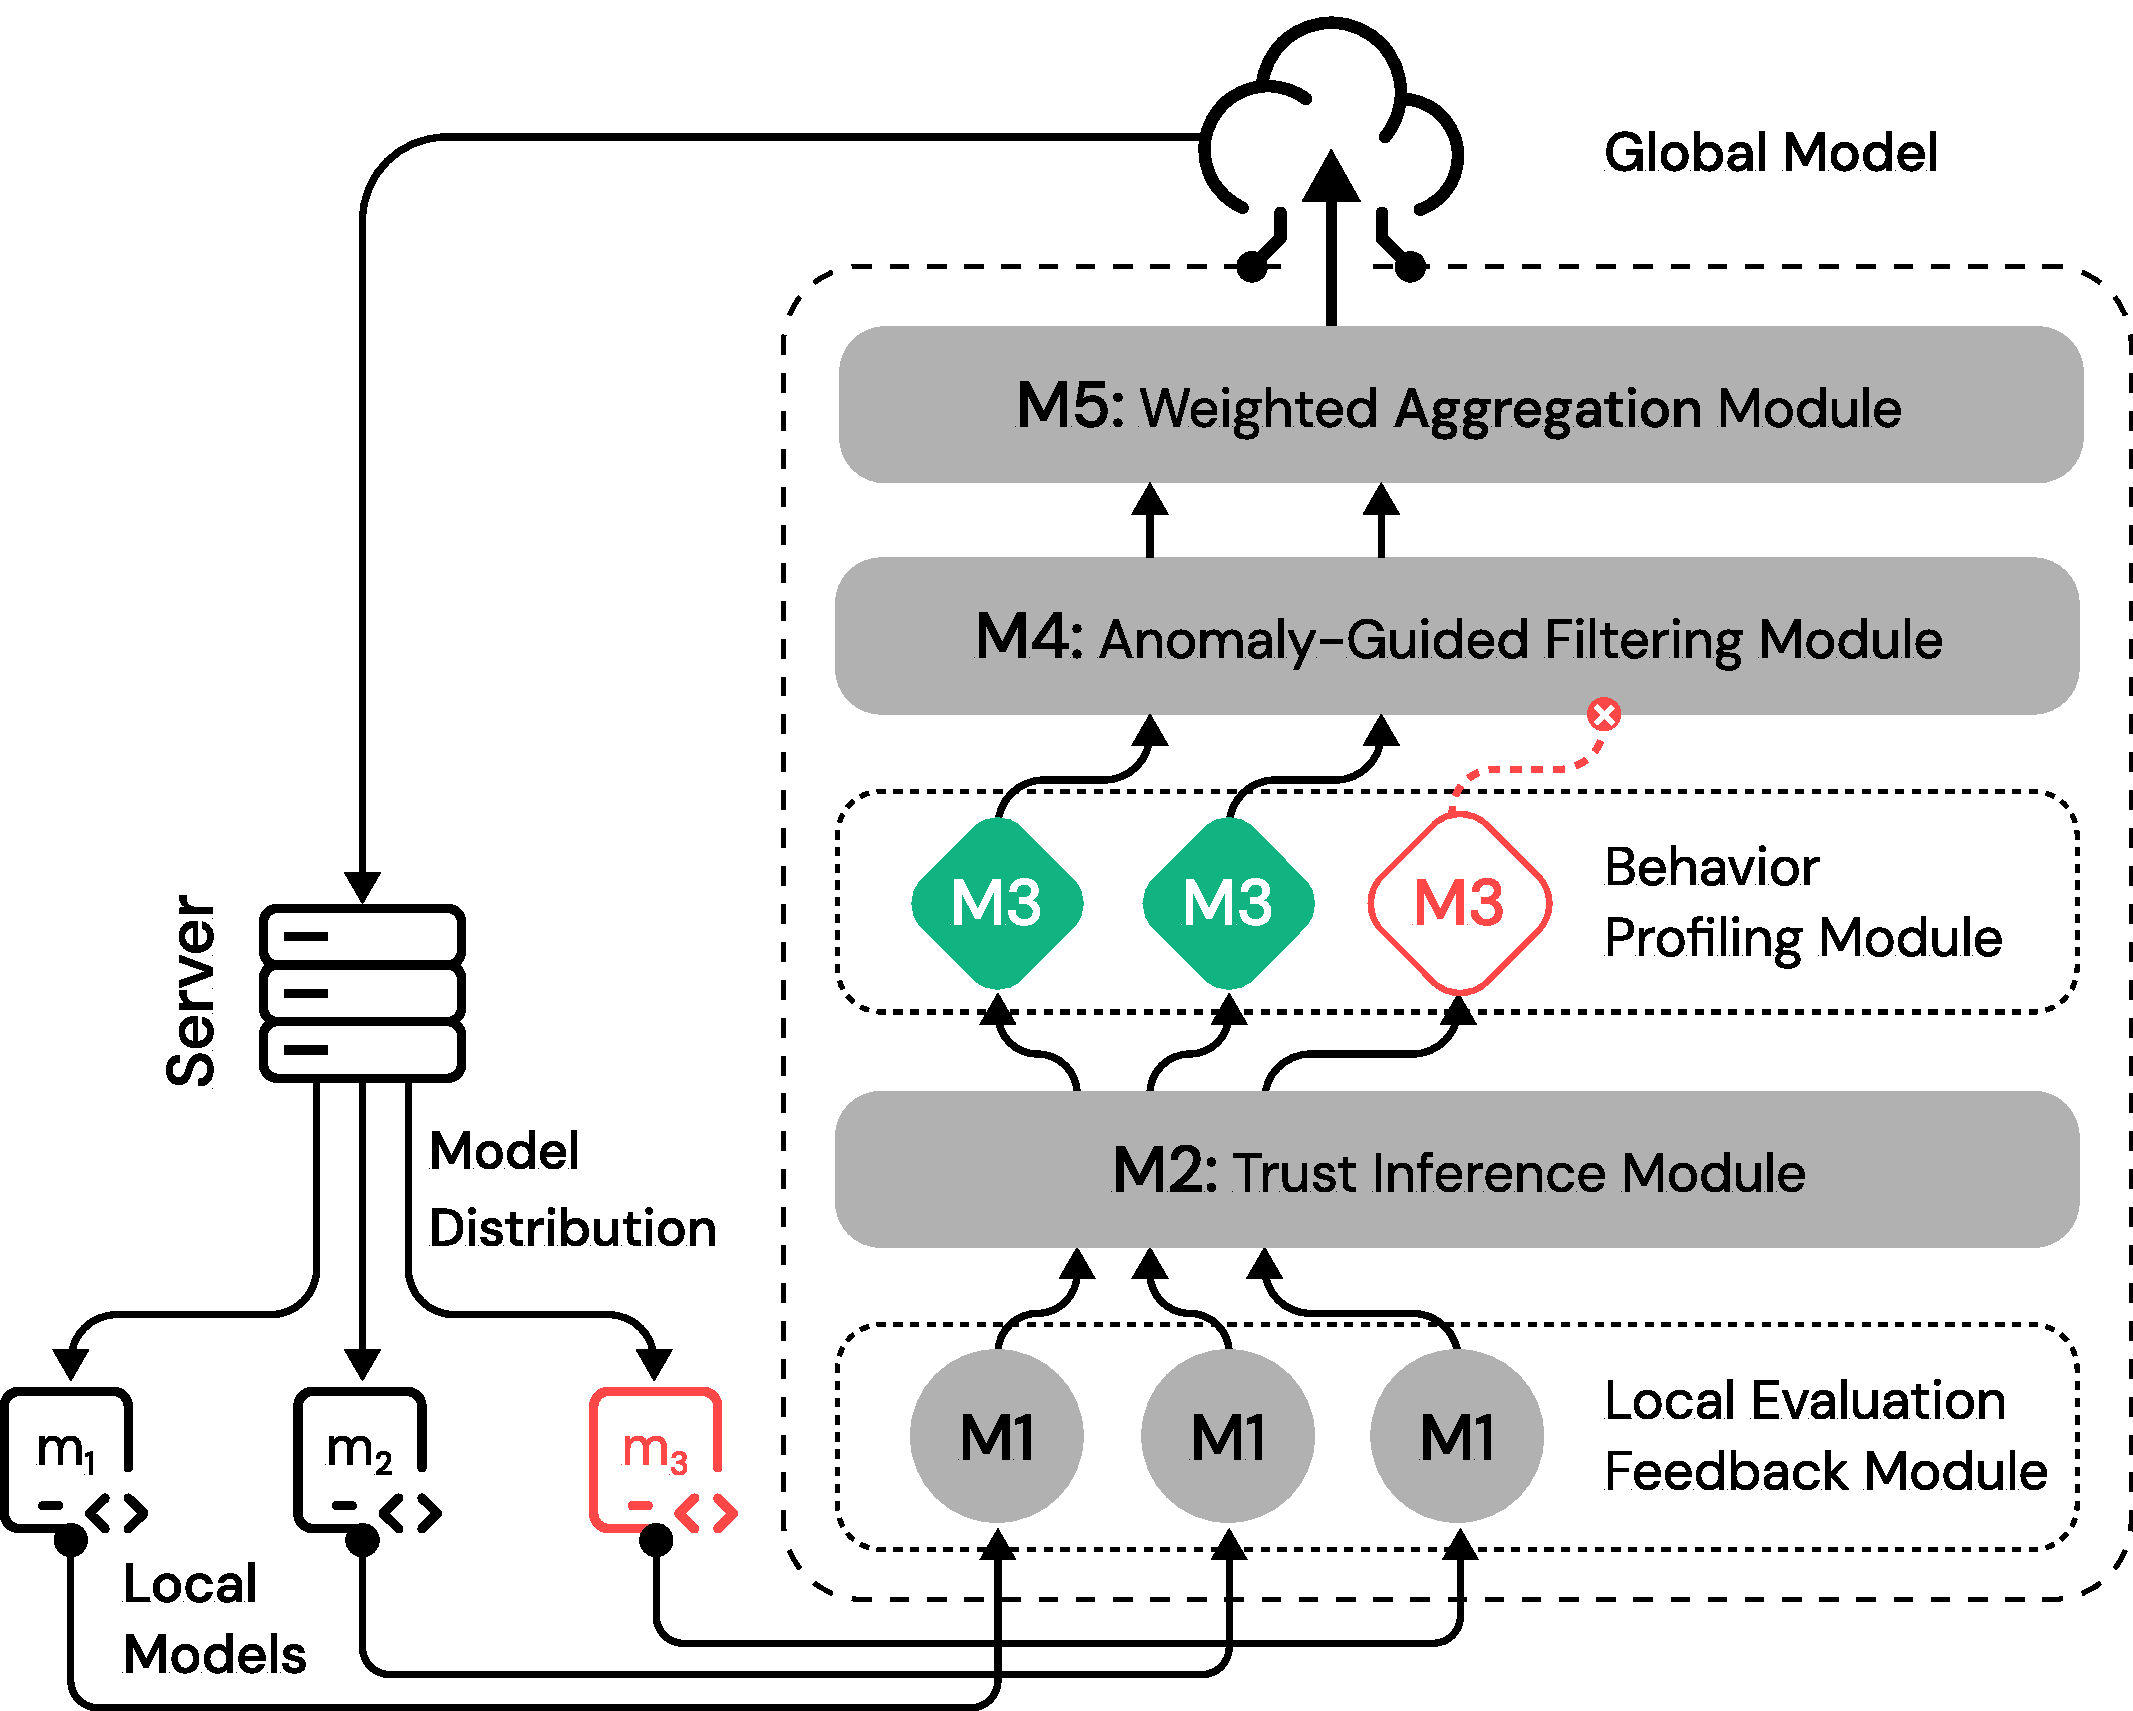
\includegraphics[width=0.9\columnwidth]{fig/sys_arc.pdf}
\caption{AntiFLipper workflow. AntiFLipper-CC adds the consistency check (M3) between the reports and the trust update.}
\label{fig:arch}
\end{figure}

\textbf{M1 -- Local evaluation report.} Before local training, client $j$ evaluates $M_t$ on a fraction $\gamma$ of its local data and uploads $a_{j,t}$ (4 bytes) with $m_{j,t}$. An honest flipper evaluates on the labels it trains on; a report-faking flipper evaluates on its true labels.

\textbf{M2 -- Trust update.} With $\bar a_t$ the mean report, trust moves by the squared deviation:
\begin{equation}
\tau_j \leftarrow \max\!\big(0,\ \tau_j + \operatorname{sgn}(a_{j,t}-\bar a_t)\,\eta\,(a_{j,t}-\bar a_t)^2\big),
\label{eq:trust}
\end{equation}
followed by normalization over the non-excluded clients. The quadratic form ignores small fluctuations and reacts strongly to large gaps.

\textbf{M3 -- Update-consistency check (new).} Let $\delta_j$ be the change of the last layer (weights and bias) of client $j$ in round $t$, and $\tilde\delta$ the coordinate-wise median of all $\delta_j$. The server computes $s_j=\cos(\delta_j,\tilde\delta)$ and the robust score $r_j=(s_j-\operatorname{med}(s))/(1.4826\,\operatorname{MAD}(s))$. A client with $r_j<-z$ is \emph{inconsistent}: its report is replaced by $\min_i a_{i,t}$ before (\ref{eq:trust}), and it receives a flag in M4 regardless of its trust. The intuition is that relabelling class $k$ as $\pi(k)$ pushes the classifier row of $\pi(k)$ towards features of class $k$ and vice versa. The resulting last-layer change opposes that of honest clients, who own the same classes. The median is computed coordinate-wise, so it is not determined by any minority of clients.

\textbf{M4 -- Flagging and exclusion.} After $g=2$ warm-up rounds, client $j$ is flagged when its trust falls below a fixed share of the uniform weight, $n_t\,\tau_j<\rho$, or when M3 marks it inconsistent. Flags are cumulative, and a client with $c_j\ge c_{\max}$ flags is excluded from the round in which this happens onward. The relative threshold makes $\rho$ independent of the number of clients; the absolute threshold of earlier versions was not.

\textbf{M5 -- Weighted aggregation.} $M_{t+1}=\sum_{j\notin\beta}\tau_j\,m_{j,t}\big/\sum_{j\notin\beta}\tau_j$, where $\beta$ is the set of excluded clients.

\textbf{Ablations.} \emph{AntiFLipper (reports)} omits M3. \emph{CC only} omits M1--M2: trust stays uniform, and only M3 flags lead to exclusion.

\setlength{\textfloatsep}{6pt}
\begin{algorithm}[t]
\caption{AntiFLipper-CC, server side of round $t$}
\label{alg:cc}
\small
\KwIn{models $m_{j,t}$ and reports $a_{j,t}$ of clients $j\notin\beta$; trust $\tau$; counters $c$}
$\tilde\delta\leftarrow$ coordinate-wise median of last-layer updates $\delta_j$\;
\ForEach{$j\notin\beta$}{ $s_j\leftarrow\cos(\delta_j,\tilde\delta)$ }
$I\leftarrow\{j: (s_j-\operatorname{med}(s))/(1.4826\operatorname{MAD}(s))<-z\}$\;
\lForEach{$j\in I$}{$a_{j,t}\leftarrow\min_i a_{i,t}$}
update $\tau$ with (\ref{eq:trust}); normalize over $j\notin\beta$\;
\If{$t\ge g$}{
 \ForEach{$j\notin\beta$}{
  \lIf{$n_t\tau_j<\rho$ \textbf{or} $j\in I$}{$c_j\leftarrow c_j+1$}
  \lIf{$c_j\ge c_{\max}$}{$\beta\leftarrow\beta\cup\{j\}$}
 }
 normalize $\tau$ over $j\notin\beta$\;
}
\Return $M_{t+1}=\sum_{j\notin\beta}\tau_j m_{j,t}$, $\tau$, $c$, $\beta$
\end{algorithm}

% =============================================================================
% Full-width floats are placed one page early so they appear next to Section VI.
\begin{table*}[t]
\centering
\caption{Final test accuracy (\%, mean$\pm$std over 3 seeds) with 40\% label-flipping clients, and server-side defense time per round on CIFAR-10 non-IID. $^\dagger$FLTrust additionally uses a 100-sample clean root dataset at the server. -- : not run in this setting or not yet completed.}
\label{tab:headline}
\renewcommand{\arraystretch}{1.12}
\small
\begin{tabular}{l|cc|cc|c}
\hline
& \multicolumn{2}{c|}{\textbf{CIFAR-10 (ResNet-18, 20 clients)}} & \multicolumn{2}{c|}{\textbf{MNIST (CNN, 100 clients)}} & \textbf{Defense time} \\
\textbf{Method} & non-IID ($\alpha_D{=}1$) & IID & non-IID ($\alpha_D{=}1$) & IID & (ms, CIFAR non-IID) \\
\hline
FedAvg & 17.50$\pm$2.28 & 52.61$\pm$36.38 & 33.83$\pm$56.11 & 0.63$\pm$0.21 & 34.2$\pm$0.7 \\
Median & 60.29$\pm$2.98 & 60.00$\pm$5.73 & -- & -- & 355.7$\pm$4.4 \\
Multi-Krum & 48.98$\pm$37.19 & 72.64$\pm$0.24 & -- & -- & 875.1$\pm$12.0 \\
FLAME & 58.88$\pm$14.05 & 71.03$\pm$0.55 & -- & -- & 1058.5$\pm$13.4 \\
LFighter & 50.54$\pm$24.36 & 73.41$\pm$0.07 & 98.49$\pm$0.11 & 98.74$\pm$0.11 & 41.7$\pm$3.8 \\
FLTrust$^\dagger$ & 71.15$\pm$0.57 & 70.70$\pm$3.99 & 97.27$\pm$0.03 & 97.54$\pm$0.16 & 351.8$\pm$4.1 \\
\hline
CC only & 68.40$\pm$5.24 & -- & -- & -- & 24.5$\pm$0.3 \\
AntiFLipper-CC & 70.48$\pm$0.10 & 71.85$\pm$1.22 & 98.66$\pm$0.11 & 98.71$\pm$0.15 & 23.4$\pm$0.6 \\
AntiFLipper (reports) & 71.12$\pm$0.30 & 73.28$\pm$0.25 & 98.67$\pm$0.10 & 98.71$\pm$0.15 & 23.5$\pm$0.8 \\
AntiFLipper-CR+CC & -- & -- & -- & -- & -- \\
\textbf{AntiFLipper-CR} & -- & -- & -- & -- & -- \\
\hline
\end{tabular}
\end{table*}

\begin{figure*}[t]
\centering
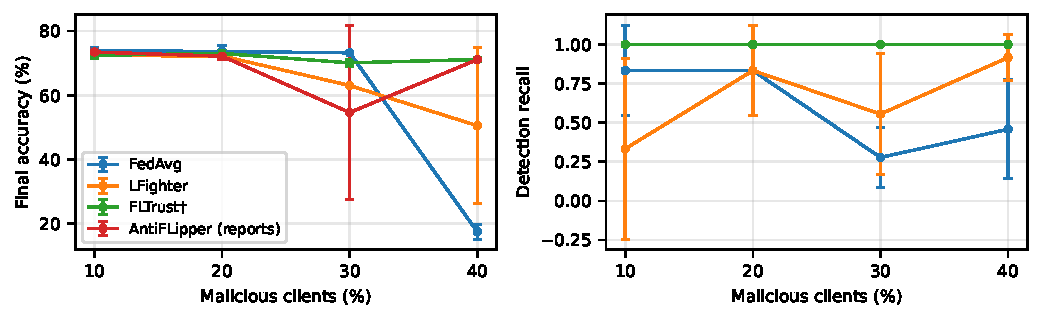
\includegraphics[width=0.85\textwidth]{fig/gen_ratio.pdf}
\caption{Final accuracy (left) and detection recall (right) on CIFAR-10 non-IID as the share of malicious clients grows to the 40\% threat-model bound (mean$\pm$std over 3 seeds).}
\label{fig:ratio}
\end{figure*}
\begin{figure*}[t]
\centering
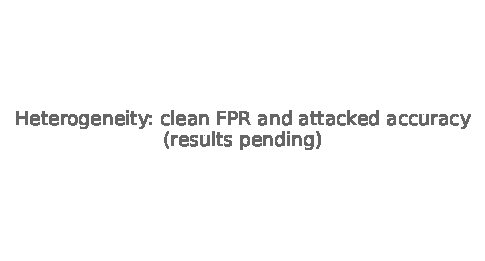
\includegraphics[width=0.85\textwidth]{fig/gen_heterogeneity.pdf}
\caption{Left: false-positive rate without attackers as data become more skewed ($\alpha_D$ from 1 to 0.1). Right: final accuracy with 40\% attackers at $\alpha_D=0.1$ (CIFAR-10, 3 seeds).}
\label{fig:het}
\end{figure*}
\section{Analysis}
\label{sec:analysis}
% =============================================================================
\begin{proposition}[Report signal]\label{prop:signal}
Let $a_H$ and $a_M=a_H-g$ be the expected accuracy of $M_t$ on honest and on flipped local labels, with $g>0$. With honest reporting, a flipper's expected deviation from the mean is $-(1-p)g$ and an honest client's is $+pg$.
\end{proposition}
\emph{Proof.} $\mathbb{E}[\bar a]=(1-p)a_H+pa_M=a_H-pg$; subtract from $a_M$ and $a_H$. \hfill$\square$

Under (\ref{eq:trust}), flippers therefore lose trust in expectation and honest clients gain it. The separation shrinks linearly in $p$ and vanishes if the global model itself becomes poisoned ($g\to 0$), one reason we bound $p\le 0.4$.

\begin{proposition}[Report faking defeats report-only detection]\label{prop:faking}
If every flipper reports the accuracy of $M_t$ on its unflipped labels, the reports of flippers and honest clients with identically distributed data have the same distribution. No rule that depends on the reports alone can then separate them better than chance.
\end{proposition}
\emph{Proof.} A faked report is computed by the same function of $(M_t, x, y)$ on the same distribution as an honest report; only the training labels differ, and they do not enter the report. \hfill$\square$

Under non-IID data the two distributions differ only through the data split, which carries no information about who flips. Detection therefore needs a signal derived from what the client \emph{did}, its update, which M3 provides.

\begin{proposition}[Consistency check]\label{prop:cc}
Suppose fewer than half of the clients flip and honest last-layer updates are concentrated around a direction $u$. Then the coordinate-wise median $\tilde\delta$ stays within the range of the honest coordinates, and a flipper whose update satisfies $\cos(\delta_j,u)<\cos(\delta_h,u)$ for typical honest $h$ obtains a lower similarity score $s_j$.
\end{proposition}
\emph{Argument.} The coordinate-wise median has breakdown point $1/2$~\cite{yin2018byzantine}, so with $p<1/2$ each median coordinate lies between honest values. Flipping class $k$ to $\pi(k)$ reverses the sign of the cross-entropy gradient on the logit rows of $k$ and $\pi(k)$ for the affected samples, which lowers the alignment of $\delta_j$ with $u$. The claim is conditional: strong heterogeneity widens the spread of honest $s_h$ and can push honest clients below the cut-off. We therefore measure the false-positive rate without attackers at $\alpha_D\in\{0.1,0.5,1\}$ (Fig.~\ref{fig:het}). Partial flips weaken the signal. \hfill$\square$

\begin{proposition}[Finite exclusion]
A client that is flagged in $c_{\max}$ rounds after warm-up is excluded no later than its $c_{\max}$-th flagged round.
\end{proposition}
This bounds the damage an identified attacker can do. It does not imply that every flagged client is malicious, which Tables~\ref{tab:detection} and~\ref{tab:sensitivity} measure.

\textbf{Cost.} Training costs $\approx 3E\,|D_j|$ forward passes; the report adds $\gamma|D_j|$, i.e.\ a relative client overhead of $\gamma/(3E)\approx 11\%$ for $\gamma=1$, $E=3$ (1.1\% for $\gamma=0.1$). Table~\ref{tab:cost} reports the measured ratio. The upload grows by 4 bytes per round, a fraction $1/W$ of a $W$-parameter float32 model (below $10^{-4}$ for both models used here). On the server, M3 costs $O(n_t d_L)$ for the median and similarities, plus $O(n_t\log n_t)$ for the robust score. Multi-Krum costs $O(n_t^2 W)$, FLAME computes $n_t^2$ cosine similarities in dimension $W$ and clusters them, and FLTrust trains a root model each round.

\textbf{Privacy.} A scalar report reveals far less than an update, but repeated reports describe how well the global model fits a client's data. Calibrated noise on $a_{j,t}$ is a natural mitigation; M3 does not use the reports and is unaffected by it. Quantifying this trade-off is future work.

\textbf{Convergence.} M5 is a convex combination of surviving models with history-dependent weights. Standard FedAvg guarantees~\cite{li2020convergence} hold for the surviving population once exclusions stop, but false exclusions change that population. We report per-round accuracy and surviving-client counts from the logs as empirical evidence.

% =============================================================================
\section{Evaluation}
\label{sec:eval}
% =============================================================================
\subsection{Setup}
\textbf{Data and models.} We use CIFAR-10 with ResNet-18, 20 clients and 100 rounds, and MNIST with a 21{,}840-parameter CNN, 100 clients and 200 rounds. The client counts follow the original evaluation and are the same for IID and non-IID splits. Non-IID splits draw class proportions per client from $\mathrm{Dir}(\alpha_D)$, with $\alpha_D=1$ unless stated otherwise. All clients participate in every round. Clients run $E=3$ epochs of SGD (learning rate 0.01, momentum 0.9, weight decay $5\cdot10^{-4}$, batch 32 for CIFAR-10 and 64 for MNIST).

\textbf{Attack.} Unless stated otherwise, 40\% of the clients flip all of their labels with $\pi$ in every round, and report honestly.

\textbf{Baselines.} FedAvg, coordinate-wise Median, Multi-Krum ($f=\lfloor pN\rfloor$), FLAME, LFighter and FLTrust. FLTrust receives a balanced root set of 100 clean samples held out from all clients, an advantage the other methods do not have. All methods share the same partitions, attackers and seeds.

\textbf{Hyperparameters.} AntiFLipper variants use $\eta=0.1$, $\rho=0.05$, $c_{\max}=6$, $g=2$, $z=2.5$ and $\gamma=1$. Sensitivity runs use three held-out seeds (101, 113, 127) that are not used for any reported comparison; all comparisons use seeds 7, 19 and 31.

\textbf{Metrics.} Final-round test accuracy (mean$\pm$std over seeds); attack success rate (ASR), the share of test predictions equal to $\pi(y)$; precision, recall and false-positive rate of the identified clients; mean exclusion round; server defense time per round (pre-aggregation checks plus aggregation, excluding FLTrust's root training, which is reported separately); measured client report and training time; and peak memory. Timings come from runs with two jobs per GPU. Relative comparisons share these conditions, and a separate fixed-workload benchmark gives matched-$N$ aggregation times.

\subsection{Main comparison}
Table~\ref{tab:headline} compares final accuracy across the four settings, and Table~\ref{tab:detection} reports attack impact and identification on the main setting, CIFAR-10 non-IID.
\pending{state where AntiFLipper-CC ranks against LFighter and FLTrust in accuracy and defense time; whether its accuracy is within one std of the best method; how the CC-only and reports-only ablations compare to the combination.}

\begin{table}[t]
\centering
\caption{Attack impact and attacker identification on CIFAR-10 non-IID (40\% attackers, mean over 3 seeds). ASR: share of test predictions equal to the flipped label. P/R/FPR: final precision, recall and false-positive rate of the excluded (AntiFLipper variants) or zero-weighted (baselines) clients. Det.: mean round at which an attacker is excluded.}
\label{tab:detection}
\renewcommand{\arraystretch}{1.1}
\footnotesize
\setlength{\tabcolsep}{3.5pt}
\begin{tabular}{l|c|ccc|c}
\hline
\textbf{Method} & \textbf{ASR (\%)} & \textbf{P} & \textbf{R} & \textbf{FPR} & \textbf{Det.} \\
\hline
FedAvg & 59.6 & n/a & n/a & n/a & n/a \\
Median & 14.5 & n/a & n/a & n/a & n/a \\
Multi-Krum & 24.6 & 0.60 & 0.75 & 0.33 & n/a \\
FLAME & 15.6 & 0.49 & 0.42 & 0.17 & n/a \\
LFighter & 23.7 & 0.71 & 0.46 & 0.08 & n/a \\
FLTrust$^\dagger$ & 4.2 & 0.60 & 0.92 & 0.44 & n/a \\
CC only & 4.1 & 0.86 & 1.00 & 0.11 & 11.2 \\
AntiFLipper-CC & 3.3 & 0.73 & 1.00 & 0.25 & 12.8 \\
AntiFLipper (reports) & 3.3 & 0.90 & 1.00 & 0.08 & 15.0 \\
AntiFLipper-CR+CC & -- & -- & -- & -- & -- \\
\textbf{AntiFLipper-CR} & -- & -- & -- & -- & -- \\
\hline
\end{tabular}
\end{table}


\subsection{Report-faking attacker}
\begin{table}[t]
\centering
\caption{Report-faking adaptive attacker on CIFAR-10 non-IID: attackers train on flipped labels but report the accuracy measured on their clean labels. Methods that do not use reports are unaffected, so their honest-report runs apply to both columns.}
\label{tab:adaptive}
\renewcommand{\arraystretch}{1.1}
\footnotesize
\setlength{\tabcolsep}{4pt}
\begin{tabular}{l|cc|cc}
\hline
& \multicolumn{2}{c|}{\textbf{Honest reports}} & \multicolumn{2}{c}{\textbf{Faked reports}} \\
\textbf{Method} & Acc. (\%) & Recall & Acc. (\%) & Recall \\
\hline
LFighter & -- & -- & -- & -- \\
FLTrust$^\dagger$ & -- & -- & -- & -- \\
CC only & -- & -- & -- & -- \\
AntiFLipper (reports) & -- & -- & -- & -- \\
\textbf{AntiFLipper-CC} & -- & -- & -- & -- \\
\hline
\end{tabular}
\end{table}

Table~\ref{tab:adaptive} repeats the main setting with report-faking attackers. A preliminary 8-round MNIST run (10 clients, 4 attackers) illustrates the effect. Report-only AntiFLipper excluded 2/4 honest-reporting attackers but 0/4 report-faking attackers, and its accuracy fell from 95.6\% to 79.8\%. AntiFLipper-CC excluded 4/4 in both cases with no false positives (95.6\% and 95.7\%).
\pending{CIFAR-10 numbers over three seeds; confirm that report-only recall collapses and AntiFLipper-CC recall is preserved.}

\begin{figure}[t]
\centering
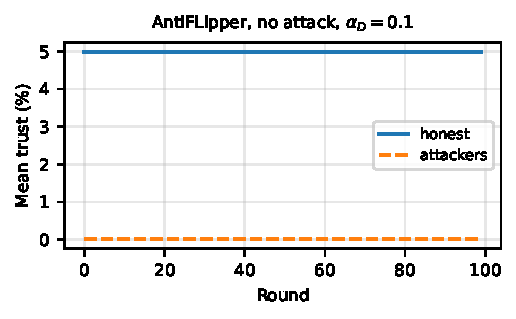
\includegraphics[width=\columnwidth]{fig/gen_trajectories.pdf}
\caption{Mean trust of honest clients and attackers under report faking (CIFAR-10 non-IID, seed 7). Report-only trust cannot separate the groups; with the consistency check the attackers are flagged and excluded.}
\label{fig:traj}
\end{figure}

\subsection{Malicious ratio}
Fig.~\ref{fig:ratio} varies $p$ from 10\% to 40\%. Prop.~\ref{prop:signal} predicts a report gap that shrinks with $p$, while Prop.~\ref{prop:cc} holds for any $p<1/2$.
\pending{the ratio at which report-only recall first drops, and whether AntiFLipper-CC keeps recall and accuracy up to 40\%.}

\subsection{Heterogeneity and false positives}
Fig.~\ref{fig:het} measures the main risk of the consistency check: honest clients with very skewed data also produce atypical last-layer updates.
\pending{FPR of each variant at $\alpha_D=0.1$ and the accuracy ranking under attack at $\alpha_D=0.1$.}

\subsection{Sensitivity and cost}
\begin{table}[t]
\centering
\caption{One-factor sensitivity of AntiFLipper-CC on MNIST non-IID (held-out seeds). Attack: 40\% flippers; clean: no attackers, so every exclusion is a false positive.}
\label{tab:sensitivity}
\renewcommand{\arraystretch}{1.1}
\footnotesize
\begin{tabular}{l|cc|c}
\hline
& \multicolumn{2}{c|}{\textbf{Attack}} & \textbf{Clean} \\
\textbf{Setting} & Acc. (\%) & Recall & FPR \\
\hline
default ($\rho{=}0.05$, $c_{\max}{=}6$, $z{=}2.5$) & -- & -- & -- \\
$\rho=0.025$ & -- & -- & -- \\
$\rho=0.1$ & -- & -- & -- \\
$c_{\max}=3$ & -- & -- & -- \\
$c_{\max}=9$ & -- & -- & -- \\
$z=2.0$ & -- & -- & -- \\
$z=3.0$ & -- & -- & -- \\
\hline
\end{tabular}
\end{table}

\begin{table}[t]
\centering
\caption{Measured cost per round for AntiFLipper-CC (mean over seeds). Client: report evaluation vs.\ local training time per client and their ratio. Server: defense time (cross-check, trust update and aggregation) and peak GPU memory of the job. Upload: extra bytes over FedAvg per client.}
\label{tab:cost}
\renewcommand{\arraystretch}{1.1}
\scriptsize
\setlength{\tabcolsep}{2.5pt}
\begin{tabular}{l|ccc|cc|c}
\hline
& \multicolumn{3}{c|}{\textbf{Client}} & \multicolumn{2}{c|}{\textbf{Server}} & \\
\textbf{Setting} & Eval & Train & Ratio & Defense & GPU & \textbf{Upl.} \\
 & (s) & (s) & (\%) & (ms) & (MB) & \\
\hline
CIFAR non-IID & -- & -- & -- & -- & -- & -- \\
CIFAR IID & -- & -- & -- & -- & -- & -- \\
MNIST non-IID & -- & -- & -- & -- & -- & -- \\
MNIST IID & -- & -- & -- & -- & -- & -- \\
\hline
\end{tabular}
\end{table}

Table~\ref{tab:sensitivity} varies one hyperparameter at a time around the defaults, with and without attackers. Table~\ref{tab:cost} reports the measured client overhead, which can be compared with the analytical $\gamma/(3E)$, and the server cost of the check.
\pending{the range over which accuracy and recall are stable; the measured overhead ratio compared with the analytical 11\%.}

% =============================================================================
\section{Limitations}
\label{sec:limits}
% =============================================================================
\begin{itemize}
\item \textbf{Threat model.} We assume at most 40\% flippers that train honestly on their (relabelled) data. Attackers that also craft their updates to align with the median can evade M3; robust aggregation against such model poisoning is complementary.
\item \textbf{Adaptive attacks.} Partial flips reduce both signals. Colluding attackers that coordinate their updates are not evaluated.
\item \textbf{Scope.} Image classification with two architectures and synchronous full participation. Client timings come from a GPU workstation rather than edge hardware.
\item \textbf{Statistics.} Three seeds per setting support mean$\pm$std but not fine-grained significance claims.
\end{itemize}

% =============================================================================
\section{Conclusion}
\label{sec:conclusion}
% =============================================================================
A defense that trusts client-reported accuracy is cheap and needs no server data, but a client can lie about the report, and a report-only defense cannot detect the lie. AntiFLipper-CC keeps the cheap report and adds a last-layer consistency check that makes lying detectable, at negligible server and communication cost.
\pending{one sentence on the measured headline result.} Future work includes partial and colluding attackers, privacy-preserving reports, and deployment on edge devices.

\bibliographystyle{IEEEtran}
\bibliography{IEEEabrv,bibliography_updated}
\end{document}
